%\documentclass[fontsize=12pt, paper=a4]{report}
\documentclass[fontsize=12pt, paper=a4]{scrreprt}
%\documentclass[fontsize=12pt, paper=a4, headinclude, twoside=false, parskip=half+, pagesize=auto, numbers=noenddot, plainheadsepline, open=right]{scrreprt}
%\documentclass[11pt,a4paper]{article}
%\usepackage[latin1]{inputenc}
\usepackage[utf8]{inputenc}
\usepackage[T1]{fontenc}
%\usepackage[ngerman]{babel}
\usepackage[ngerman,english]{babel}
\usepackage[square,numbers]{natbib}
\usepackage{textcomp}
\usepackage{lmodern}

\usepackage[intlimits]{amsmath}
\usepackage{amssymb}
\usepackage{moreverb}

% PDF-Kompression
\pdfminorversion=5
\pdfobjcompresslevel=1

%\usepackage[automark]{scrpage2} % Kopf- und Fu�zeilen
%\usepackage{amsmath,marvosym} % Mathesachen
%\usepackage{mathpazo} % Palatino f�r Mathemodus
%\usepackage{mathpazo,tgpagella} % auch sehr sch�ne Schriften

\usepackage{setspace} % Zeilenabstand
\onehalfspacing % 1,5 Zeilen

% Schriften-Gr��en
\setkomafont{chapter}{\Large\rmfamily}
\setkomafont{section}{\large\rmfamily}
\setkomafont{subsection}{\normalsize\rmfamily}
\setkomafont{subsubsection}{\normalsize\rmfamily}
\setkomafont{paragraph}{\rmfamily}
\setkomafont{subparagraph}{\rmfamily}
%\setkomafont{chapterentry}{\large\rmfamily}
%\setkomafont{descriptionlabel}{\bfseries\rmfamily}
\setkomafont{captionlabel}{\upshape\bfseries}
\setkomafont{caption}{\itshape}

\usepackage[ngerman,english,pdfauthor={Andreas Mantler}, pdftitle={Design of a Semi-Actuated Tangible Device for Tabletop Interface Interactions}, breaklinks=true]{hyperref}
\usepackage[final]{microtype}
\usepackage{url}
\usepackage{multirow}
\usepackage{multicol}
\usepackage{tabularx}
\usepackage{longtable}
\usepackage{array}
\usepackage{float}
\usepackage{graphicx}
\usepackage{color}

\graphicspath{{images/}}
\DeclareGraphicsExtensions{.pdf,.png,.jpg}
\renewcommand{\thefigure}{\arabic{figure}}
\renewcommand{\thetable}{\arabic{table}}
\usepackage{subcaption}
\usepackage{rotating}
%\newcommand{\subfigureautorefname}{\figurename}
\usepackage[all]{hypcap}
%\setcapindent{0em}
%\setcapwidth[c]{0.9\textwidth}
%\setlength{\abovecaptionskip}{0.2cm}
\usepackage{chngcntr}
\counterwithout{figure}{chapter}

\usepackage{listings}
\usepackage{color}

\definecolor{mycomment}{rgb}{0,0.6,0}
\definecolor{mygray}{rgb}{0.5,0.5,0.5}
\definecolor{mymauve}{rgb}{0.58,0,0.22}

\lstset{ %
  backgroundcolor=\color{white},   % choose the background color; you must add \usepackage{color} or \usepackage{xcolor}
  basicstyle=\footnotesize,        % the size of the fonts that are used for the code
  breakatwhitespace=false,         % sets if automatic breaks should only happen at whitespace
  breaklines=true,                 % sets automatic line breaking
  commentstyle=\color{mycomment},  % comment style
  deletekeywords={...},            % if you want to delete keywords from the given language
  escapeinside={\%*}{*)},          % if you want to add LaTeX within your code
  extendedchars=true,              % lets you use non-ASCII characters; for 8-bits encodings only, does not work with UTF-8
  frame=single,                    % adds a frame around the code
  keepspaces=true,                 % keeps spaces in text, useful for keeping indentation of code (possibly needs columns=flexible)
  keywordstyle=\color{blue},       % keyword style
  language=C++,                    % the language of the code
%  otherkeywords={*,...},           % if you want to add more keywords to the set
  numbers=left,                    % where to put the line-numbers; possible values are (none, left, right)
  numbersep=5pt,                   % how far the line-numbers are from the code
  numberstyle=\tiny\color{mygray}, % the style that is used for the line-numbers
  rulecolor=\color{black},         % if not set, the frame-color may be changed on line-breaks within not-black text (e.g. comments (green here))
  showspaces=false,                % show spaces everywhere adding particular underscores; it overrides 'showstringspaces'
  showstringspaces=false,          % underline spaces within strings only
  showtabs=false,                  % show tabs within strings adding particular underscores
  stepnumber=1,                    % the step between two line-numbers. If it's 1, each line will be numbered
  stringstyle=\color{mymauve},     % string literal style
  tabsize=2,                       % sets default tabsize to 2 spaces
  title=\lstname                   % show the filename of files included with \lstinputlisting; also try caption instead of title
}
%\lstset{
%	extendedchars=true,
%	basicstyle=\tiny\ttfamily,
%	tabsize=2,
%	keywordstyle=\textbf,
%	commentstyle=\color{gray},
%	stringstyle=\textit,
%	numbers=left,
%	numberstyle=\tiny,
%	breakautoindent  = true,
%	breakindent      = 2em,
%	breaklines       = true,
%	postbreak        = ,
%	prebreak         = \raisebox{-.8ex}[0ex][0ex]{\Righttorque},
%}

% linksb�ndige Fu�boten
\deffootnote{1.5em}{1em}{\makebox[1.5em][l]{\thefootnotemark}}

\typearea{14}

\makeatletter
\newcommand{\saved@equation}{}
\let\saved@equation\equation
\def\equation{\@hyper@itemfalse\saved@equation}
\makeatother

% einr�cken nach �berschriften
\makeatletter
\let\@afterindentfalse\@afterindenttrue % Absatzeinzug auch nach �berschriften
\@afterindenttrue
\makeatother

\newcommand*\justify{%
  \fontdimen2\font=0.4em% interword space
  \fontdimen3\font=0.2em% interword stretch
  \fontdimen4\font=0.1em% interword shrink
  \fontdimen7\font=0.1em% extra space
  \hyphenchar\font=`\-% allowing hyphenation
}

% bild mit defnierter Breite einf�gen
\newcommand{\bild}[4]{
  \begin{figure}[!hbt]
    \centering
      \vspace{1ex}
      \includegraphics[width=#2]{images/#1}
      \caption[#4]{\label{img.#1} #3}
    \vspace{1ex}
  \end{figure}
}
% bild mit eigener Breite
\newcommand{\bilda}[3]{
  \begin{figure}[!hbt]
    \centering
      \vspace{1ex}
      \includegraphics{images/#1}
      \caption[#3]{\label{img.#1} #2}
      \vspace{1ex}
  \end{figure}
}

\font\texttrm = cmr17
\font\textttrm = cmr17 at 13pt

\addtolength{\textwidth}{-15mm}
\addtolength{\oddsidemargin}{13mm}

\addtolength{\headheight}{6.5mm}
\addtolength{\headsep}{0mm}%-24.5mm}
\addtolength{\textheight}{5mm}%28.5mm}
\addtolength{\footskip}{-7.5mm}

\usepackage[headsepline, footsepline, plainheadsepline]{scrpage2}
\pagestyle{scrheadings}
\clearscrheadfoot
\renewcommand*{\chaptermarkformat}{}
%\renewcommand*{\sectionmarkformat}{}
\automark[section]{chapter}
\renewcommand*{\chapterheadstartvskip}{\vspace{-11mm}}
\renewcommand*{\chapterheadendvskip}{\vspace{4mm}}

\setlength{\parindent}{0mm}

% punkte im Inhaltsverzeichnis
\makeatletter
\renewcommand*\l@chapter[2]{
  \ifnum \c@tocdepth >\m@ne
    \addpenalty{-\@highpenalty}
    \vskip 1.0em \@plus\p@
    \setlength\@tempdima{1.5em}
    \begingroup
      \parindent \z@ \rightskip \@pnumwidth
      \parfillskip -\@pnumwidth
      \leavevmode \bfseries
      \advance\leftskip\@tempdima
      \hskip -\leftskip
      #1\nobreak\normalfont\leaders\hbox{$\m@th
        \mkern \@dotsep mu\hbox{.}\mkern \@dotsep
        mu$}\hfill\nobreak\hb@xt@\@pnumwidth{\hss\bf #2}\par
      \penalty\@highpenalty
    \endgroup
  \fi}

%\renewcommand\l@section[2]{
%  \ifnum \c@tocdepth >\z@
%    \addpenalty\@secpenalty
%    \addvspace{1.0em \@plus\p@}
%    \setlength\@tempdima{1.5em}
%    \begingroup
%      \parindent \z@ \rightskip \@pnumwidth
%      \parfillskip -\@pnumwidth
%      \leavevmode \bfseries
%      \advance\leftskip\@tempdima
%      \hskip -\leftskip
%      #1\nobreak\ 
%      \leaders\hbox{$\m@th\mkern \@dotsep mu\hbox{.}\mkern \@dotsep mu$}
%     \hfil \nobreak\hb@xt@\@pnumwidth{\hss #2}\par
%    \endgroup
%  \fi}
%\makeatother

% newline after \paragraph
\makeatletter
\renewcommand\paragraph{%
   \@startsection{paragraph}{4}{0mm}%
      {-\baselineskip}%
      {.01\baselineskip}%
      {\normalfont\normalsize\bfseries}}
\makeatother

\AtBeginDocument{\addtocontents{toc}{\protect\thispagestyle{empty}}}



\begin{document}

	% Titelseite
	\begin{center}
		\vspace*{54mm}
		{
			\renewcommand{\baselinestretch}{0.9}\normalsize
			\Large
			\textbf{Oculus Meets AR - Documentation}\\
		}
		\vspace*{15.5mm}
		{
			\large
			\textbf{Project Seminar}\\
		}
		\vspace*{10mm}
		{
			at\\
			\textbf{Westfälischen Wilhelms-Universität Münster}\\
		}
		\vspace*{100mm}
		\begin{tabular*}{137mm}{ll}
			Authors: 		& \textbf{Tim Michels }, Matr.Nr. 348072\\
						& \textbf{Florian Kleene}, Matr.Nr. 374601\\
						& \textbf{Christian Thiele}, Matr.Nr. 374531\\
						& \textbf{Andreas Mantler}, Matr.Nr. 363220\\
			Submission date: 	& 20 April 2015
		\end{tabular*}
	\end{center}
	\newpage
	
	% Leere Seite
	\thispagestyle{empty}\quad\newpage
	
	% Inhaltsverzeichnis
	\thispagestyle{empty}
	\tableofcontents
	\addtocontents{toc}{\vspace{-5mm}}
	\vfill
	\newpage

	% Leere Seite
	\thispagestyle{empty}\quad\newpage
	
	% Inhalt
	\setcounter{page}{1}
	\pagestyle{scrheadings}
	\setfootsepline{0pt} 
	\ihead[\chaptername\ \thechapter: \leftmark]{\chaptername\ \thechapter: \leftmark}
	\cfoot[\vspace*{9mm}\pagemark]{\vspace*{9mm}\pagemark}
	\renewcommand{\baselinestretch}{1.3}\normalsize

	\chapter{Introduction}
	\label{sec:introduction}
	The aim of this project is to equip the Oculus Rift DK2 with a stereo camera system and build a framework in order to extend its functionality regarding AR (augmented reality). While AR applications using smartphones or wearables like Google Glass are only able to augment a small part of our FOV (field of view), head mounted displays (HMD) like Oculus Rift are not limited in this regard and are therefore creating a more immersive experience. Furthermore the use of a HMD enables the user to switch between VR (virtual reality) and AR.\\
In addition we integrate a tracking system, which enables us to get the exact position of the HMD as well as the position of any other object equipped with so-called rigid bodies. This allows interactions with the virtual objects supplemented to the real-world environment without using further input devices.

\section*{Previous Work}
There are mainly two similar (published) projects to ours. The first one is the commercial \href{http://ovrvision.com/}{OVRVision} by Shinobiya.com Co.Ltd., which is available for Oculus Rift DK2. The OVRVision has two fixed, parallel mounted cameras and therefore lacks the option to adjust the position of these cameras to match the user's IPD (interpupillary distance). Secondly there is William Steptoe's well documented project \href{http://willsteptoe.com/post/66968953089/ar-rift-part-1}{AR-Rift}, which is more flexible regarding the cameras' positions, but is based on the Oculus Rift DK1, which has a much lower resolution than the DK2 used for our project. Nevertheless our project is built upon ideas of both these AR-extensions for Oculus Rift.	

	\chapter{Hardware Requirements}
	\label{sec:hardware_requirements}
	Please note that every single part of the following hardware
configuration is optional in the example applications. You do not need
any of the hardware present to develop with ARLib! This is the hardware we were
developing for:
\begin{itemize}
	\item{2x \href{http://www.logitech.com/de-de/product/hd-webcam-c310}{Logitech C310 Webcams}}
	\item{\href{https://github.com/ands/OculusMeetsAR/tree/master/Hardware/Printmodels}{3D-Printed camera mounts and lens mounts}}
	\item{2x \href{http://www.camera2000.com/en/cctv-board-security-video-camera-1-8mm-lens-f2-0.html}{Fisheye 1.8mm lens F2.0}}
	\item{\href{https://www.oculus.com/dk2/}{Oculus Rift DK2 Head-Mounted Display}}
	\item{\href{http://www.optitrack.com/products/flex-3/}{OptiTrack Flex 3 Tracking System}}
\end{itemize}

\begin{figure}[htb!]
	\centering
	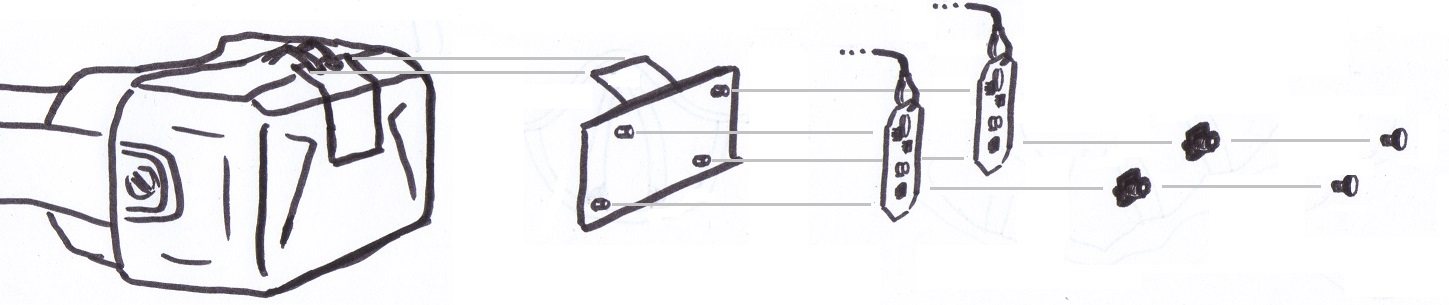
\includegraphics{explosion}
	\vspace{1mm}
	\caption{Exploded-view drawing of our modified HMD. The components from left to right: Oculus Rift DK2, 3D-printed camera mount, Logitech C310s, 3D-printed lens mounts, lenses.}
	\label{fig:explosion}
\end{figure}

\subsection{Lens selection and camera calibration}\label{lens-selection-and-camera-calibration}

Regarding our hardware choices we recommend William Steptoe's
\href{http://willsteptoe.com/post/67399683294/ar-rift-camera-selection-part-2}{documentation
on his project AR-Rift}. According to different user-reports, the actual
horizontal FOV of the DK2, which should be matched by the lenses, is
only about 80\textdegree-90\textdegree. With our lenses, we got a vertical* FOV of
approximately 75\textdegree, so for a more accurate matching one might want to buy
lenses with a smaller focal length. To prevent easy mistakes on your
search for other lenses, we recommend
\href{http://pomeroyprinting.blogspot.de/2014/04/modifying-logitech-c310-hd-webcam.html}{this
post by Brandon Pomeroy}.

For calibration we used Davide Scaramuzzas
\href{https://sites.google.com/site/scarabotix/ocamcalib-toolbox}{OCamCalib toolbox} along with a small
\href{https://github.com/ands/OculusMeetsAR/tree/master/Hardware}{stereo calibration tool}, we implemented using OpenCV. Click
\href{https://github.com/ands/OculusMeetsAR/wiki/Calibration}{here} for a step-by-step guide and technical details.
\\
\\
*Remark: This is the relevant FOV since the cameras are mounted with a 90\textdegree rotation!
	
	\chapter{Stereo Calibration}
	\label{sec:stereo_calibration}
	\begin{center}
\textbf{Developed by Tim Michels}
\end{center}
\begin{enumerate}
\item 
Before starting the stereo calibration, download the \href{https://sites.google.com/site/scarabotix/ocamcalib-toolbox}{OCamCalib Toolbox} for Matlab provided by Davide Scaramuzza\cite{ocamcalib}. Use this tool to calculate the intrinsic camera parameters for both cameras. We recommend our calibration tool to take snapshots for both cameras (see 3). Rename the two resulting calib\_results.txt to calib\_results\_CAM1.txt (left camera) and calib\_results\_CAM2.txt (right camera) and place these files at /Hardware/Calibration\_Tool/media/
\item
  Connect your webcams to the system and start our
  \href{https://github.com/ands/OculusMeetsAR/tree/master/Hardware/Calibration_Tool}{calibration
  tool}. You will see the main menu.
	
  \includegraphics*[width=.92\textwidth]{0.jpg}
	
  Note: We built our system for two Logitech C310 webcams with Logitech
  drivers installed. If you don't want to use Logitech Cxxx cameras or
  the Logitech drivers, you will have to modify the
  \href{https://github.com/ands/OculusMeetsAR/tree/master/ARLib/src/Video}{VideoPlayer.cpp}.
\item
  Take snapshots, which you can use for the stereo calibration (main
  menu option 1). After selecting this option, press SPACE to take
  snapshot or ESC to exit.
\item
  Load the images from the media folder (main menu option 2). The tool
  will list the snapshots.
	
  \includegraphics*[width=.92\textwidth]{2.jpg}
	
  Now select the snapshots, you want to use for calibration (simply
  press ENTER to select all). Here we decided to choose the snapshot
  pairs 1,2,3,4 and 7. Then our tool loads and undistorts (according to
  the previously determined ocam models) the images.
	
  \includegraphics*[width=.92\textwidth]{3.jpg}
	
\item
  Extract and match keypoints (main menu option 3).
	
  \includegraphics*[width=.92\textwidth]{4.jpg}
	
  Select the second option and choose the method for keypoint extraction
  and matching -
  \href{http://en.wikipedia.org/wiki/Scale-invariant_feature_transform}{SIFT}\cite{sift},
  chessboard detection (using OpenCV's chessboard corner detector), or a
  combination of both.
	
  \includegraphics*[width=.92\textwidth]{5.jpg}
	
  If you choose the first or last method, you will have the option to
  check the matches manually.
	
  \includegraphics*[width=.92\textwidth]{6.jpg}
	
  If you want to examine the matches manually, for every match you will
  get an image like this.
	
  \includegraphics*[width=.92\textwidth]{7.jpg}
	
  Now press the RIGHT ARROW KEY to accept the currently displayed match
  or any other key to reject it. After matching the keypoints of an
  image pair, the console will tell you, how many matches you accepted
  and how many of those were added to the final collection of matches.
  Some correct matches might be discarded because of previously added
  very similar matches.
	
  \includegraphics*[width=.92\textwidth]{8.jpg}
	
  For chessboard matching you need to enter the number of inner
  chessboard corners (e.g.~for a standard 8x8 chessboard enter 7 as
  x-size as well as y-size).
	
  \includegraphics*[width=.92\textwidth]{9_0.jpg}
	
\item
  Approximate the
  \href{http://en.wikipedia.org/wiki/Epipolar_geometry}{epipolar
  geometry}\cite{epipolar} (main menu option 4). With the calculated or selected
  matches we now want to estimate the fundamental matrix as well as the
  homographies, which we can use to rectify our camera streams.
	
  \includegraphics*[width=.92\textwidth]{9_1.jpg}
	
  Here we used two methods: 1. The implementation of Hartley's
  \href{http://docs.opencv.org/modules/calib3d/doc/camera_calibration_and_3d_reconstruction.html\#findfundamentalmat}{8-point-algorithm}\cite{hartley8point}
  from OpenCV, which uses RANSAC for more than 8 points. 2. We
  implemented
  \href{http://publica.fraunhofer.de/documents/N-246139.html}{\emph{Joint estimation of epipolar geometry and rectification parameters using point correspondences for stereoscopic TV sequences}} by Zilly, Mueller, Eisert and Kauff\cite{joint_estimation}.
	
  \includegraphics*[width=.92\textwidth]{10.jpg}
	
  If you choose the latter, you can calculate the rectifying
  homographies either according to the mentioned paper or using
  \href{http://docs.opencv.org/modules/calib3d/doc/camera_calibration_and_3d_reconstruction.html\#stereorectifyuncalibrated}{OpenCV's
  implementation of Hartley's algorithm}\cite{hartley}.
	
  \includegraphics*[width=.92\textwidth]{11.jpg}
	
\item
  Visualize the approximated fundamental matrix and homographies (main
  menu option 5). This will draw some epipolar lines on the first image
  pair loaded. Furthermore it will rectify theses images. The results
  are saved to the media folder.
	
  \includegraphics*[width=.92\textwidth]{12.jpg}
	
\item
  If you are satisfied with the results, you will have to copy the files
  homography\_CAM1.txt and homography\_CAM2.txt from the media folder to
  ARLibSamples/media/.
\end{enumerate}
	
	\chapter{Framework Overview}
	\label{sec:lib_overview}
	\section{ARLib}\label{arlib}

This is the main library we are developing here. It is comprised of the
following modules:

\begin{itemize}
\item
  \hyperref[sec:video_library]{ARLibVideo}:
  The stereo video input library. It grabs real-time video streams from
  the two cameras\cite{c310} attached to the Oculus Rift DK2\cite{dk2} and provides
  coordinate lookup tables to undistort them according to their lens
  parameters and align them to one another according to their
  precalculated homographies.
\item
  \hyperref[sec:oculus_library]{ARLibOculus}:
  A small wrapper for LibOVR\cite{dk2}. Only the needed parts. It initializes the
  HMD, provides the LibOVR configuration parameters and the latest
  LibOVR tracking data.
\item
  \hyperref[sec:tracking_library]{ARLibTracking}:
  The rigid body tracking library. It uses the NatNetSDK\cite{optitrack} and/or
  ARLibOculus to provide the latest positions and orientations of rigid
  bodies as well as a fraction of their tracking history for retroactive
  queries.
\item
  \hyperref[sec:ogre_library]{ARLibOgre}:
  The OGRE 1.9\cite{ogre} interface library. This is the only part of ARLib that depends on
  OGRE. It provides all the shaders, materials, render targets and
  abstracted components that can be directly inserted into a scene.
\end{itemize}

\section{ARLib\_Samples}\label{arlibux5fsamples}

We provide two simple example projects that demonstrate the usage of
ARLib within OGRE:

\begin{itemize}
\item
  \hyperref[sec:simple_scene]{SimpleScene}:
  A simple example scene with some static objects placed around the
  origin.
\item
  \hyperref[sec:remote_game]{RemoteGame}:
  A simple game where one has to defend against laser bullets of a \emph{Star
  Wars Remote}.
\end{itemize}
	
	\chapter{Video Library}
	\label{sec:video_library}
	\begin{center}
\textbf{Developed by Tim Michels}
\end{center}
In order to grab the video from the two Logitech C310 webcams we used the capture
class from Microsofts Media Foundation example
\href{https://msdn.microsoft.com/en-us/library/windows/desktop/ee663604\%28v=vs.85\%29.aspx}{MFCaptureToFile Sample}\cite{mfcapturetofile}
and modified
\href{https://github.com/ands/OculusMeetsAR/blob/master/ARLib/src/Video/CCapture.cpp}{it}.
If you want to use different cameras, video resolution or drivers,
you'll have to modify this class (especially the ConfigureSourceReader
function, where we set the video format). Furthermore you'll need to
modify the camera selection in the constructor of
\href{https://github.com/ands/OculusMeetsAR/blob/master/ARLib/src/Video/videoplayer.cpp}{VideoPlayer.cpp}.

However if you just want to use the video module with two C310\cite{c310} and the
drivers provided by Logitech, you'll just have to create a VideoPlayer
instance via the following constructor:
\begin{lstlisting}
VideoPlayer(int cameraNumber = 0, const char *ocamModelParametersFilename = NULL, float videoDistance = 4.0f, const char *homographyMatrixFilename = NULL);
\end{lstlisting}
In order to undistort the video (using the ocam parameters mentioned in
the \hyperref[sec:stereo_calibration]{calibration section}) and rectify it according to a previously approximated homography, you need to hand over the filenames. Furthermore we used cameraNumber 0 for the left and 1 for the right camera. The videoDistance is similar to a zoom factor applied to the video. To see its effect, look at:
\begin{lstlisting}
void calculateUndistortionMap(float *xyMap);
// map size: getVideoWidth() * getVideoHeight() * sizeof(float) * 2
\end{lstlisting}

After initialization the videoPlayer will immediately start capturing.
To get a pointer to the current video frame memory in the BGR format, you then just have to call videoPlayer's following methods:
\begin{lstlisting}
LARGE_INTEGER captureTimeStamp;
void *frameData = videoPlayer->beginUpdate(&captureTimeStamp);
// use the frameData here if it is not NULL.
// frame size: getVideoWidth() * getVideoHeight() * 3
videoPlayer->endUpdate();
\end{lstlisting}
The captureTimeStamp is optional. If you provide a captureTimeStamp to beginUpdate and frameData is not NULL, it will be filled with the timestamp at which the frame arrived.

\newpage
\section{Tips \& Problem solving}\label{tips-problem-solving}

\begin{itemize}
\itemsep1pt\parskip0pt\parsep0pt
\item
  One camera can be attached to the built-in USB port of the Oculus Rift DK2, if the DK2s additional power supply is used.
\item
  We couldn't get more than one video stream over that built-in USB port. The second camera needs a separate USB cord.
\item
  Sometimes, the Logitech driver enables a digital zoom (Probably to lower the amount of data transferred over a USB root hub). Try a different USB port for one of the cameras.
\item
  Camera enumeration seems to happen in exactly the same order each time.
\end{itemize}
	
	\chapter{Oculus Library}
	\label{sec:oculus_library}
	\begin{center}
\textbf{Developed by Andreas Mantler}
\end{center}
ARLibOculus is just a lightweight single-class wrapper for the needed parts of LibOVR (the Oculus SDK)\cite{dk2}.
Including \href{https://github.com/ands/OculusMeetsAR/blob/master/ARLib/include/ARLib/Oculus/Rift.h}{ARLib/Oculus/Rift.h} won't pull any LibOVR header files into the compilation unit.
In fact, it doesn't depend on anything at all!

\section{\texorpdfstring{\href{https://github.com/ands/OculusMeetsAR/blob/master/ARLib/include/ARLib/Oculus/Rift.h}{ARLib::Rift}}{ARLib::Rift}}\label{arlibrift}
\texttt{ARLib::Rift} has some static methods as well as non-static ones.
The static methods are needed to initialize and shutdown the LibOVR system as a whole,
while the non-static methods operate on single instances of Oculus Rift devices.

\subsubsection{Static Methods}\label{static-methods}

\begin{lstlisting}
static void init();
\end{lstlisting}
Initializes LibOVR. Must be called once before using anything else from ARLibOculus.

\begin{lstlisting}
static void shutdown();
\end{lstlisting}
Shuts down LibOVR. Should be called once after deleting all \texttt{ARLib::Rift} instances.

\begin{lstlisting}
static bool available(int id);
\end{lstlisting}
Test if an Oculus Rift device with the specified id is connected (0 is the first connected Rift).

\subsubsection{Methods}\label{methods}

\begin{lstlisting}
enum RIFT_ERROR_CODE
{
    RIFT_OK,
    RIFT_CONNECTION_ERROR,
    RIFT_TRACKING_ERROR
};

RIFT_ERROR_CODE initialize(int id);
\end{lstlisting}
Initializes the instance. Tries to connect to the Oculus Rift device with the specified id. Returns \texttt{RIFT\_OK} on success.

\begin{lstlisting}
void getTextureSizes(
    int *size2dL,
    int *size2dR);
\end{lstlisting}
Writes the recommended render target texture/framebuffer resolutions for each eye into the specified \texttt{int{[}2{]}} arrays.

\begin{lstlisting}
void getUVScalesAndOffsets(
    float *scale2dL, float *offset2dL,
    float *scale2dR, float *offset2dR);
\end{lstlisting}
Writes texture coordinate shader parameters for each eye to the specified \texttt{float{[}2{]}} arrays.
These have to be passed as uniforms to the \href{https://github.com/ands/OculusMeetsAR/blob/master/ARLib/ogre_media/ARLibOculusDistortionVertex.glsl}{ARLibOculusDistortionVertex.glsl} shader.

\begin{lstlisting}
struct DistortionVertex
{
    // [-1,+1],[-1,+1] over the entire framebuffer:
    float ScreenPosNDC[2];

    // Lerp factor between time-warp matrices. Can be encoded in Pos.z:
    float TimeWarpFactor; 

    // Vignette fade factor. Can be encoded in Pos.w:
    float VignetteFactor;

    // Chromatic aberration correction parameters:
    float TanEyeAnglesR[2];
    float TanEyeAnglesG[2];
    float TanEyeAnglesB[2];
};

void getDistortionGeometries(
    DistortionVertex **verticesL, int *vertexNumL,
    unsigned short **indicesL, int *indexNumL,
    DistortionVertex **verticesR, int *vertexNumR,
    unsigned short **indicesR, int *indexNumR);
\end{lstlisting}
Writes pointers to triangle mesh data and data quantities for the distortion meshes of each eye to the specified locations.

\begin{lstlisting}
void getProjections(
    float znear, float zfar, bool rightHanded,
    float *aspectRatioL, float *projection4x4L,
    float *aspectRatioR, float *projection4x4R);
\end{lstlisting}
For specified near and far distances, writes device aspect ratios and projection matrices for each eye into the specified locations.

\begin{lstlisting}
void getPose(float *position3d, float *orientationQuaternionXYZW);
\end{lstlisting}
Writes the latest LibOVR tracking position and orientation to the specified \texttt{float{[}3{]}} and \texttt{float{[}4{]}} arrays.

\begin{lstlisting}
void recenterPose();
\end{lstlisting}
Will recenter the tracking position and orientation (yaw component) to the current pose.

\begin{lstlisting}
float getInterpupillaryDistance();
\end{lstlisting}
Returns the configured IPD (interpupillary distance) for the current LibOVR user.

\begin{lstlisting}
bool isPositionCurrentlyTracked();
bool isOrientationCurrentlyTracked();
bool isCameraPoseCurrentlyTracked();
bool isPositionTrackingConnected();
\end{lstlisting}
Various LibOVR tracking state flags.
	
	\chapter{Tracking Library}
	\label{sec:tracking_library}
	\begin{center}
\textbf{Developed by Florian Kleene \& Christian Thiele}
\end{center}
The Tracking Library supports several methods for real-time pose determination and estimation. Along with the tracking devices included in the Oculus Rift (both DK1 and DK2\cite{dk2}), any device using the NatNetSDK\cite{optitrack} is supported. The core of this Module is the \texttt{TrackingManager} class. It is practically the only necessary interface to fire-up an application with tracking support. The proper use of the tracking library will be discussed in the following sections.
\section{Initialization of the Tracking Manager}\label{tracking-manager-initialization}

Initialization of the tracking manager requires the user to hand over the necessary parameters to the TrackingManager beforehand. First of all we create an instance of the class while also defining its purpose.

\begin{lstlisting}
TrackingManager tManager = TrackingManager(ARLib::ARLIB_NATNET | ARLib::ARLIB_RIFT, frameBufferSize, debugOutput);
\end{lstlisting}
where frameBufferSize determines the buffer size for retroactive queries (more on that later) and debugOutput is a boolean value enabling debug console output. In this example the tracking manager is set up to connect to a NatNet Server (i.e Motive etc.) as well as reading tracking data from the rifts inertial sensors, providing more stability in the tracking data (there is also support for multiple rifts).
The \texttt{initialize} function returns the status of the tracking manager. This is very helpfull for debugging. Furthermore the tracking manager should not be used unless no error is returned by the \texttt{initialize} function.

\begin{lstlisting}
if(ARLib::ARLIB_TRACKING_OK != tManager->initialize()){
    printf("Failed to Initialize Tracking Manager.");
    return -1;
}
\end{lstlisting}
Depending on wether the tracking is critical for your application or not you should exit your program.

\section{Using the Tracking Manager}\label{using-the-tracking-manager}

The tracking manager needs to be updated on a regular basis (i.e. your event-loop), if your are using the Oculus Rift. For smooth transformations, this should happen at least 75 times per second, that is the frame rate supported by the Oculus DK2, or 60 times per second for the DK1.

To make objects behave according to the tracking data (i.e. ridig body transformations) they have to inherit from the abstract base class \texttt{RigidBodyEventListener}. On each event cycle the manager will notify its listeners of any change in their transformations. A \texttt{RigidBodyEventListener} has a, not necessarily unique, ID, which is used to create a correspondence between the rigid bodies on the server (Motive etc.) and the rigid bodies in your application.

For the Oculus there is a specialized \texttt{RigidBodyEventListener} the \texttt{\justify RiftRigidBodyEventListener}. The \texttt{RiftSceneNode} from the OgreModule is such a specialized listener. On Registration with the Tracking Manager, a handle to the rift is saved and queried for positional data each frame.


\section{Retroactive Queries}\label{retroactive-queries}

The camera images need to be placed in front of the virtual camera, which is of course a representative of the Oculus. But to reduce the effect of latency, which is naturally imposed by the webcams, the images need to be placed where they were at capture time. This solution works rather nicely in situations where the camera motion is not particularly fast. When the camera is moving faster the user will experience black borders at the edge of the screen, because the images could not cover the whole rendering area. To query the position of the RiftRigidBodyEventListener one must call the function.

\begin{lstlisting}
RigidBody* TrackingManager::evaluateRigidBody(unsigned int ID, const long long& retroActiveQuery);
\end{lstlisting}

ID is of course the RigidBody identifier, and retroActiveQuery is the desired Timestamp formated equavalently to the QueryPerformanceCounter function.

\section{Cleaning Up}\label{cleaning-up}

If the Tracking Manager is no longer used simply delete the handle to it. The cleanup will be taken care of by the destructor.
		
	\chapter{Ogre Library}
	\label{sec:ogre_library}
	\begin{center}
\textbf{Developed by Andreas Mantler}
\end{center}
ARLibOgre provides an engine-dependent integration of ARLib into the \emph{Object oriented Graphics Rendering Engine (OGRE)}\cite{ogre}.

\section{Example}\label{example}

Usage in an OGRE scene (have a look at the
\href{https://github.com/ands/OculusMeetsAR/tree/master/ARLib_Samples}{ARLib\_Samples}
for more details):

\begin{lstlisting}
// create a rift node and add it to the tracking system
riftNode = new ARLib::RiftSceneNode(
    rift, sceneManager, 0.001f, 50.0f, 1);
tracker->addRigidBodyEventListener(riftNode);

// add a render target that renders to the rift screen (window)
renderTarget = new ARLib::RiftRenderTarget(rift, root, window);
riftNode->addRenderTarget(renderTarget);

// add a render target that renders to an additional debug output
smallRenderTarget = new ARLib::DebugRenderTarget(smallWindow);
riftNode->addRenderTarget(smallRenderTarget);

// attach video screens (call riftVideoScreens->update() each frame!)
riftVideoScreens = new ARLib::RiftVideoScreens(sceneManager,
    riftNode, leftVideoPlayer, rightVideoPlayer, tracker);
\end{lstlisting}

\section{Class Listing}
ARLibOgre is comprised of the following classes:

\newpage
\subsubsection{\texorpdfstring{\href{https://github.com/ands/OculusMeetsAR/blob/master/ARLib/include/ARLib/Ogre/RiftSceneNode.h}{ARLib::RiftSceneNode}
: public
\href{https://github.com/ands/OculusMeetsAR/blob/master/ARLib/include/ARLib/Tracking/RigidBodyEventListener.h\#L33}{ARLib::RiftRigidBodyEventListener}}{ARLib::RiftSceneNode : public ARLib::RiftRigidBodyEventListener}}\label{arlibriftscenenode-public-arlibriftrigidbodyeventlistener}

The \texttt{RiftSceneNode} represents the virtual Oculus Rift device in the OGRE
scene. Especially, it contains the two cameras which represent the eyes.
\texttt{RenderTargets} can be connected to the \texttt{RiftSceneNode}.

\begin{lstlisting}
// constructor
RiftSceneNode(ARLib::Rift *rift, Ogre::SceneManager *sceneManager,
    float zNear, float zFar, unsigned int rigidBodyID);

// the various parts the RiftSceneNode is comprised of
ARLib::Rift *getRift();
Ogre::SceneNode *getBodyNode();
Ogre::SceneNode *getHeadNode();
Ogre::SceneNode *getHeadCalibrationNode();
Ogre::Camera *getLeftCamera();
Ogre::Camera *getRightCamera();

// manually adjustable orientation
// useful for mouselook if no actual Oculus Rift device is connected
void setPitch(Ogre::Radian angle);
void setYaw(Ogre::Radian angle);

// maintain the render targets
void addRenderTarget(ARLib::RenderTarget *renderTarget);
void removeRenderTarget(ARLib::RenderTarget *renderTarget);
void removeAllRenderTargets();
\end{lstlisting}

\subsubsection{\texorpdfstring{\href{https://github.com/ands/OculusMeetsAR/blob/master/ARLib/include/ARLib/Ogre/RiftRenderTarget.h}{ARLib::RiftRenderTarget}
: public
\href{https://github.com/ands/OculusMeetsAR/blob/master/ARLib/include/ARLib/Ogre/RenderTarget.h}{ARLib::RenderTarget}}{ARLib::RiftRenderTarget : public ARLib::RenderTarget}}\label{arlibriftrendertarget-public-arlibrendertarget}

The \texttt{RiftRenderTarget} is the \texttt{RenderTarget} that renders to the Oculus Rift
screen (in extended desktop mode), using the provided distortion meshes,
vignetting and chromatic aberration correction.

\begin{lstlisting}
// constructor
RiftRenderTarget(ARLib::Rift *rift, Ogre::Root *root,
    Ogre::RenderWindow *renderWindow);
\end{lstlisting}

\subsubsection{\texorpdfstring{\href{https://github.com/ands/OculusMeetsAR/blob/master/ARLib/include/ARLib/Ogre/DebugRenderTarget.h}{ARLib::DebugRenderTarget}
: public
\href{https://github.com/ands/OculusMeetsAR/blob/master/ARLib/include/ARLib/Ogre/RenderTarget.h}{ARLib::RenderTarget}}{ARLib::DebugRenderTarget : public ARLib::RenderTarget}}\label{arlibdebugrendertarget-public-arlibrendertarget}

The \texttt{DebugRenderTarget} is a \texttt{RenderTarget} that renders both camera images
next to each other directly to a debug output window. Use this, if you
don't have an actual Oculus Rift connected.

\begin{lstlisting}
// constructor
DebugRenderTarget(Ogre::RenderWindow *renderWindow);
\end{lstlisting}

\subsubsection{\texorpdfstring{\href{https://github.com/ands/OculusMeetsAR/blob/master/ARLib/include/ARLib/Ogre/RiftVideoScreens.h}{ARLib::RiftVideoScreens}}{ARLib::RiftVideoScreens}}\label{arlibriftvideoscreens}

\texttt{RiftVideoScreens} manages the streaming and placement of camera images.
The camera images are placed at the location in the scene where they
have been captured (according to their capture timestamp and the Rifts'
tracking data history).

\begin{lstlisting}
// constructor
RiftVideoScreens(
    Ogre::SceneManager *sceneManager, ARLib::RiftSceneNode *riftNode,
    ARLib::VideoPlayer *videoPlayerLeft,
    ARLib::VideoPlayer *videoPlayerRight,
    ARLib::TrackingManager *trackingManager = NULL);

// use these to fine-tune the video image positions and sizes
void setOffsets(Ogre::Vector2 leftOffset, Ogre::Vector2 rightOffset);
void setScalings(Ogre::Vector2 leftScale, Ogre::Vector2 rightScale);

// call this every frame to upload the latest camera images
void update();
\end{lstlisting}

	\chapter{Postprocessing}
	\label{sec:postprocessing}
	\begin{center}
\textbf{Developed by Andreas Mantler}
\end{center}
This page explains the integration of postprocessing effects into the stereo output pipeline of ARLibOgre.

\section{GlowRenderTarget}\label{glowrendertarget}

As you can see in
\href{https://github.com/ands/OculusMeetsAR/blob/master/ARLib_Samples/RemoteGame/src/GlowRenderTarget.cpp}{GlowRenderTarget.cpp},
attaching
\hyperref[sec:ogre_library]{\texttt{RenderTargets}}
to the
\href{https://github.com/ands/OculusMeetsAR/blob/master/ARLib/include/ARLib/Ogre/RiftSceneNode.h}{\texttt{RiftSceneNode}}
can be intercepted (or decorated/wrapped as in the ``decorator
pattern'') by inserting a custom \texttt{RenderTarget} in between the
\texttt{RiftSceneNode} and the actual \texttt{RenderTarget}. In
\href{https://github.com/ands/OculusMeetsAR/blob/master/ARLib_Samples/RemoteGame/src/GlowRenderTarget.cpp}{GlowRenderTarget.cpp},
the latest viewports for both eye cameras are accessed after they were
attached to add a glow effect compositor.

\section{NPRWatercolorRenderTarget}\label{nprwatercolorrendertarget}

\href{https://github.com/ands/OculusMeetsAR/blob/master/ARLib_Samples/Common/src/NPRWatercolorRenderTarget.cpp}{NPRWatercolorRenderTarget.cpp}
demonstrates a more advanced example for postprocessing. Instead of just
directly rendering and compositing into the destination \texttt{RenderTarget},
the eye camera images are passed both blurred and unchanged to an OGRE
\texttt{MultiRenderTarget}. The blurred images are used to make voronoi-like
tilings of the input image (the brushstrokes), while edges detected in
the original images are subtracted from the voronoi tilings (sharp
outlines). The results are presented in separate scenes, which are seen
by another set of cameras. Those cameras are finally passed to the
destination \texttt{RenderTarget}.

\includegraphics*[width=.92\textwidth]{NPRWatercolorRenderTarget.png}

The whole process is a simplified version of a
\href{http://csnotes.upm.edu.my/kelasmaya/web.nsf/0/d82e709c4661ce464825766400365c4d/$FILE/p231-chen.pdf}{technique
by Chen, Turk and MacIntyre from 2008}\cite{watercolor}. The idea was that if both, real
images and rendered objects are postprocessed to look like stylized
watercolor paintings, it might be more difficult to tell them apart.
	
	\chapter{Simple Scene}
	\label{sec:simple_scene}
	\includegraphics*[width=\textwidth]{SimpleSceneThumb.png}

This is the basic example. It shows the initialization and usage of ARLib for a simple Augmented Reality task in OGRE. This example can also be used to test the hardware setup. Please note that none of the hardware components have to be connected to start this example. It will tell you in the console/logfile if there were any detected problems. To keep the example simple, only three static cubes are added to the Scene. Using the tracking system, you should be able to look and walk around them and see how stable their appearance is. Using the keybindings below, you may want to finetune the video positions and sizes as well as their constant hardware latency for a smooth experience.

\section{Keybindings}\label{keybindings-1}

\begin{itemize}
\itemsep1pt\parskip0pt\parsep0pt
\item
  \textbf{`C'}: Set the origin of the scene to the current position and
  orientation of the Oculus Rift.
\item
  \textbf{`N'}: Toggle the
  \hyperref[sec:postprocessing]{Non-Photorealistic
  Rendering watercolor postprocessing effect} on/off.
\item
  \textbf{`9'}: Increase the amount of constant video latency (for the
  retroactive positioning of video frames in the scene).
\item
  \textbf{`0'}: Decrease the amount of constant video latency (for the
  retroactive positioning of video frames in the scene).
\item
  \textbf{`Q'}: Increase the interpupillary distance in the video
  background.
\item
  \textbf{`E'}: Decrease the interpupillary distance in the video
  background.
\item
  \textbf{`CTRL'}: Eye selection. The left eye is selected by default.
  While the key is pressed, the right eye is selected.
\item
  \textbf{`D'}: Move the video placement for the selected eye to the
  right.
\item
  \textbf{`A'}: Move the video placement for the selected eye to the
  left.
\item
  \textbf{`W'}: Move the video placement for the selected eye up.
\item
  \textbf{`S'}: Move the video placement for the selected eye down.
\item
  \textbf{RIGHT}: Increase the size of the selected eye horizontally.
\item
  \textbf{LEFT}: Decrease the size of the selected eye horizontally.
\item
  \textbf{UP}: Increase the size of the selected eye vertically.
\item
  \textbf{DOWN}: Decrease the size of the selected eye vertically.
\end{itemize}
	
	\chapter{Remote Game}
	\label{sec:remote_game}
	\includegraphics*[width=\textwidth]{RemoteGameThumb.png}

You should read the notes for the \hyperref[simple_scene]{SimpleScene} first. This is the more advanced example. In addition to the \hyperref[simple_scene]{SimpleScene}, this example includes some physics and gameplay code.

\section{Keybindings}\label{keybindings}

\begin{itemize}
\itemsep1pt\parskip0pt\parsep0pt
\item
  \textbf{`V'}: Pull out the lightsaber.
\item
  \textbf{`C'}: Set the origin of the scene to the current position and
  orientation of the Oculus Rift.
\item
  \textbf{`N'}: Switch between the Glow Compositor,
  \hyperref[sec:postprocessing]{Watercolor
  postprocessing effect}, both and none of them.
\item
  \textbf{`9'}: Increase the amount of constant video latency (for the
  retroactive positioning of video frames in the scene).
\item
  \textbf{`0'}: Decrease the amount of constant video latency (for the
  retroactive positioning of video frames in the scene).
\item
  \textbf{`Q'}: Increase the interpupillary distance in the video
  background.
\item
  \textbf{`E'}: Decrease the interpupillary distance in the video
  background.
\item
  \textbf{`CTRL'}: Eye selection. The left eye is selected by default.
  While the key is pressed, the right eye is selected.
\item
  \textbf{`D'}: Move the video placement for the selected eye to the
  right.
\item
  \textbf{`A'}: Move the video placement for the selected eye to the
  left.
\item
  \textbf{`W'}: Move the video placement for the selected eye up.
\item
  \textbf{`S'}: Move the video placement for the selected eye down.
\item
  \textbf{RIGHT}: Increase the size of the selected eye horizontally.
\item
  \textbf{LEFT}: Decrease the size of the selected eye horizontally.
\item
  \textbf{UP}: Increase the size of the selected eye vertically.
\item
  \textbf{DOWN}: Decrease the size of the selected eye vertically.
\end{itemize}
	
	\newpage

	% Quellenverzeichnis
	\nocite{*}
	\addcontentsline{toc}{chapter}{Bibliography}
	\ihead[\leftmark]{\leftmark}
	\begin{thebibliography}{99}

		\bibitem{arrift} AR-RIFT, Retrieved 19 April 2015 from \url{http://willsteptoe.com/post/66968953089/ar-rift-part-1}.
		\bibitem{lenses} CCTV Board Security Video Camera 1.8mm Lens F2.0, Retrieved 19 April 2015 from \url{http://www.camera2000.com/en/cctv-board-security-video-camera-1-8mm-lens-f2-0.html}.
		\bibitem{epipolar} Epipolar geometry, Retrieved 19 April 2015 from \url{http://en.wikipedia.org/wiki/Epipolar_geometry}.
		\bibitem{hartley} Hartley's stereoRectifyUncalibrated in OpenCV, Retrieved 19 April 2015 from \url{http://docs.opencv.org/modules/calib3d/doc/camera_calibration_and_3d_reconstruction.html#stereorectifyuncalibrated}.
		\bibitem{hartley8point} Hartley's 8-point-algorithm in findFundamentalMat of OpenCV, Retrieved 19 April 2015 from \url{http://docs.opencv.org/modules/calib3d/doc/camera_calibration_and_3d_reconstruction.html#findfundamentalmat}.
		\bibitem{joint_estimation} Joint estimation of epipolar geometry and rectification parameters using point correspondences for stereoscopic TV sequences, Retrieved 19 April 2015 from \url{http://publica.fraunhofer.de/documents/N-246139.html}.
		\bibitem{c310} Logitech HD Webcam C310, Retrieved 19 April 2015 from \url{http://www.logitech.com/de-de/product/hd-webcam-c310}.
		\bibitem{mfcapturetofile} MFCaptureToFile Sample, Retrieved 19 April 2015 from \url{https://msdn.microsoft.com/en-us/library/windows/desktop/ee663604%28v=vs.85%29.aspx}.
		\bibitem{modifying_lenses} Modifying a Logitech C310 HD webcam, Retrieved 19 April 2015 from \url{http://pomeroyprinting.blogspot.de/2014/04/modifying-logitech-c310-hd-webcam.html}.
		\bibitem{ocamcalib} OCamCalib: Omnidirectional Camera Calibration Toolbox for Matlab, Retrieved 19 April 201 from \url{https://sites.google.com/site/scarabotix/ocamcalib-toolbox}.
		\bibitem{dk2} OculusVR - Development Kit 2, Retrieved 19 April 2015 from \url{https://www.oculus.com/dk2/}.
		\bibitem{ogre} OGRE, Retrieved 19 April 2015 from \url{http://www.ogre3d.org/}.
		\bibitem{optitrack} OptiTrack - Flex 3, Retrieved 19 April 2015 from \url{http://www.optitrack.com/products/flex-3/}.
		\bibitem{ovrvision} Ovrvision - High Performance Stereo Camera for Oculus Rift, Retrieved 19 April 2015 from \url{http://ovrvision.com/}.
		\bibitem{mounts} OculusMeetsAR/Hardware/Printmodels, Retrieved 19 April 2015 from \url{https://github.com/ands/OculusMeetsAR/tree/master/Hardware/Printmodels}.
		\bibitem{sift} Scale-invariant feature transform, Retrieved 19 April 2015 from \url{http://en.wikipedia.org/wiki/Scale-invariant_feature_transform}.
		\bibitem{watercolor} Watercolor Inspired Non-Photorealistic Rendering for Augmented Reality, Retrieved 19 April 2015 from \url{http://csnotes.upm.edu.my/kelasmaya/web.nsf/0/d82e709c4661ce464825766400365c4d/$FILE/p231-chen.pdf}.

	\end{thebibliography}

\end{document}
